\chapter{Technologien}
\label{chap:technologies}

%%%%%%%%%%%%%%%%%%%%%%%%%%%%%%%%%%%%%%%%%%%%%%%%%%%%%%%%%%%%
\section{Bluetooth 4.0}
\label{sec:technologies:bluetooth4}
%%%%%%%%%%%%%%%%%%%%%%%%%%%%%%%%%%%%%%%%%%%%%%%%%%%%%%%%%%%%

Die Bluetooth-Version 4.0, oder auch Bluetooth Smart genannt, wurde 2009 final spezifiziert und wird seit Ende 2010 in Endgeräten eingesetzt.
Dieser Standard beinhaltet neben dem klassischen Bluetooth, eine neue Version, mit dem Namen Bluetooth Low Energy, welche, wie der Name schon andeutet, einen sehr viel geringeren Stromverbrauch vorweißt. Dabei ist der Stromverbrauch zwischen zwei und 100 mal geringer als beim klassischen Bluetooth.


%%%%%%%%%%%%%%%%%%%%%%%%%%%%%%%%%%%%%%%%%%%%%%%%%%%%%%%%%%%%
\section{Bluetooth Low Energy}
\label{sec:technologies:bluetoothLE}
%%%%%%%%%%%%%%%%%%%%%%%%%%%%%%%%%%%%%%%%%%%%%%%%%%%%%%%%%%%%

Bluetooth Low Energy wurde Anfangs von Nokia unter dem Namen ''Wibree'' entwickelt. Die Zielsetzung dabei war es eine Technologie zu entwickeln, mit der sich Computer und Mobilgeräte schnell und einfach mit Peripherie-Geräten verbinden lassen. Das Hauptaugenmerk galt dabei dem geringen Stromverbrauch, kompakter Bauweise und den Kosten für die benötigte Hardware.
Im Jahr 2007 wurden diese Spezifikationen dann in den, sich in der Entwicklung befindenden, Bluetooth-Standard 4.0 aufgenommen und daraufhin in Bluetooth Low Energy, oder kurz BLE umbenannt.

Bluetooth Low Energy arbeitet wie das klassische Bluetooth im 2,4 GHz Band, bringt aber in der Funktionsweise einige Unterschiede mit sich.

So wurde, im Vergleich zum klassischem Bluetooth, die Datenrate von bis zu 3 Mbit/s auf maximal 1 Mbit/s reduziert. Dies führt dazu, dass BLE zum Beispiel nicht für Headsets genutzt werden kann, da die zur Verffügung stehende Übertragungsrate nicht für die Audioübertragung ausreicht.

Die Vorteile die BLE mit sich bringt, liegen vor allem in der niedrigen Latenz, welche von 100ms auf bis zu unter 3ms reduziert wurde, und, wie bereits erwähnt, der Energieverbrauch drastisch gesenkt wurde.



Bluetooth Low Energy bietet darüber hinaus eine Vielzahl sogennanter GATT-Profile (Generic Attribute Profile). Die bereitgestellten GATT-Profile sind Richtlinen für die Bluetooth-Funktionialität, sprich, welche Daten übertragen werden und in welcher Form. Dies erlaubt eine einfache und schnell Interoperabilität zwischen verschiedenen Geräten. Ein Beispiel für ein GATT-Profil wäre zum Beispiel das ''Heart Rate Profile'', welches besipielsweise die Verbindung und Kommunikation eines Pulsmessgurtes mit einem Endgerät beschreibt. So wird sichergestellt, dass dieser Gurt mit jedem Endgerät auf die selbe Weise funktioniert.




%%%%%%%%%%%%%%%%%%%%%%%%%%%%%%%%%%%%%%%%%%%%%%%%%%%%%%%%%%%%
\subsection{iBeacons}
\label{sec:technologies:bluetoothLE:ibeacons}
%%%%%%%%%%%%%%%%%%%%%%%%%%%%%%%%%%%%%%%%%%%%%%%%%%%%%%%%%%%%
Die iBeacons-Technologie wurde am 10.Juni 2014 von Apple auf der Worldwide Developers Conference vorgestellt. 
Diese basiert auf Bluetooth Low Energy und arbeitet mit einem von Apple entwickelten GATT-Profil.

Beacon bedeutet übersetzt ''Leuchtfeuer'' und die Funktionsweise der Beacons ist dem sehr ähnlich.
Einmal in Betrieb genommen, sendet das Beacon kontinuierlich ein Signal, in welchem sich Daten zur Identifizierung des Beacons befinden.

Neben den Identifikationsdaten kann das Emfangsgerät noch weitere Größen bestimmen. Es ist so zum Beispiel möglich die ungefähre Entfernung einzuschätzen. 
In der iBeacons-API sind dafür vier verschiedene Zustände definiert: \textit{Far}, \textit{Near}, \textit{Immediate} und \textit{Unknown}. Diese Werte erlauben eine grobe Entfernungseinschätzung und für eine genauere Bestimmung lässt sich noch eine weitere Kenngröße bestimmen, der \textit{Accuracy}-Wert. Dabei handelt es sich um eine ungefähre Entfernungsangabe in Metern, welche jedoch ausdrücklich nur zur Differenzierung zwischen zwei Beacons genutzt werden soll und keinesfalls eine genaue Entfernung angibt.

\begin{tabular}{p{2cm}p{5cm}p{5cm}p{4cm}}
	\\
	Daten & Format & Beschreibung & Beispiel \\ \\
	UUID & 16-stellige Hexadezimalzahl & Identifizierung & 3F4 \\
	Major & Integerzahl & Identifizierung eine Region & 12 \\
	Minor & Integerzahl & Identifizierung eines einzelnen Beacons & 132 \\
	Proximity & Drei Entfernungsstufen & Ungefähre Entfernung & Far, Near, Immediate und Unknown \\
	Accuracy & Wert in Meter & Bestimmung der ungefähren Entfernung & 1.243 m \\
	RSSI & Signalstärke in dBm & Signalstärke des emfangenen Signals & -42 dBm \\
\end{tabular}


Die von dem Beacon gesendeten Daten lassen sich mit jedem BLE-kompatiblem Gerät empfangen.



Die großen Vorteile der iBeacons sind zum einen ihr kleiner Formfaktor, welcher es erlaubt die Beacons an fast jedem beliebigem Ort anzubringen, als auch ihr geringer Stromverbrauch, der es möglich macht, die Beacons bis zu mehreren Jahren mit einer Knopfzellenbatterie zu betreiben. Der Aufbau eines solchen Beacons lässt sich in Abbildung \ref{estimote-beacon} sehr gut erkennen. Den Großteil des Beacons nimmt dabei die Batterie ein. 


%%%%%%%%%%%%%%%%%%%%%%%%%%%%%%%%%%%%%%%%%%%%%%%%%%%%%%%%%%%%
% figure of estimote beacon
%%%%%%%%%%%%%%%%%%%%%%%%%%%%%%%%%%%%%%%%%%%%%%%%%%%%%%%%%%%%
\begin{figure}[h!]
	\centering
	\begin{minipage}[t]{5cm}
		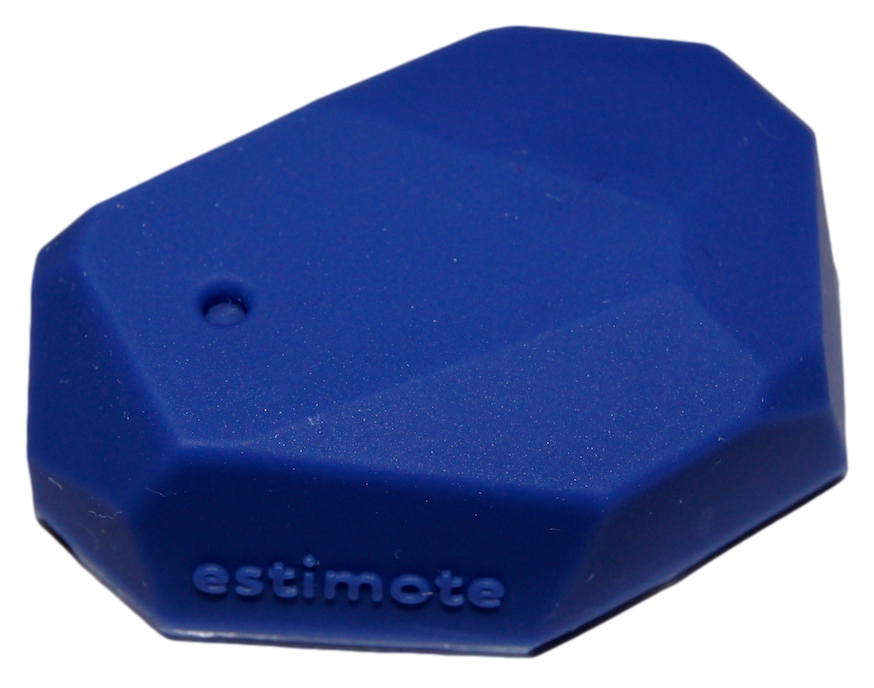
\includegraphics[scale=0.15]{pictures/estimote-beacon-outside}
		\caption{Außenhülle}
		\label{estimote-outside}
	\end{minipage}
	\hspace{2cm}
	\begin{minipage}[t]{5cm}
			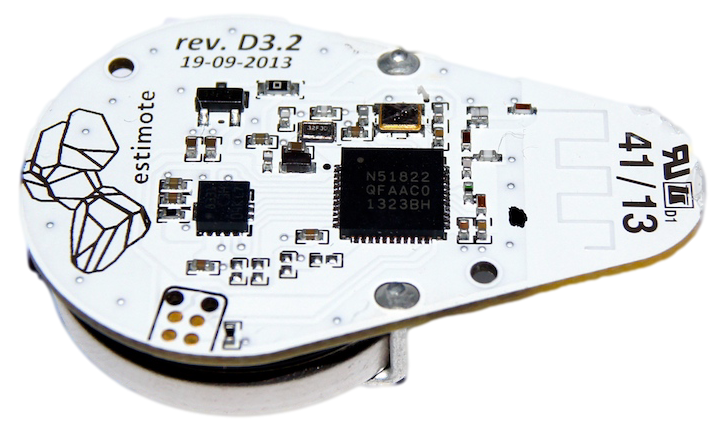
\includegraphics[scale=0.2]{pictures/estimote-beacon-inside}
			\caption{Chipsatz mit Bluetooth-Modul}
			\label{estimote-inside}
	\end{minipage}
		\caption{Ein iBeacon der Firma ''estimote''}
		\label{estimote-beacon}
\end{figure}


Unter genauerer Betrachtung des Chipsatzes in Abbildung \ref{estimote-beacon-inside-annotations}, erkennt man, dass er im Grunde aus zwei Teilen besteht.
Dem Bluetooth-Chipsatz, welcher an sich ist nur wenige Zentimeter groß und der Antenne, welche im vorderen Bereich der Platine eingearbeitet ist und die über welche letztendlich die Daten gesendet werden.

\begin{figure}[h!]
	\centering
	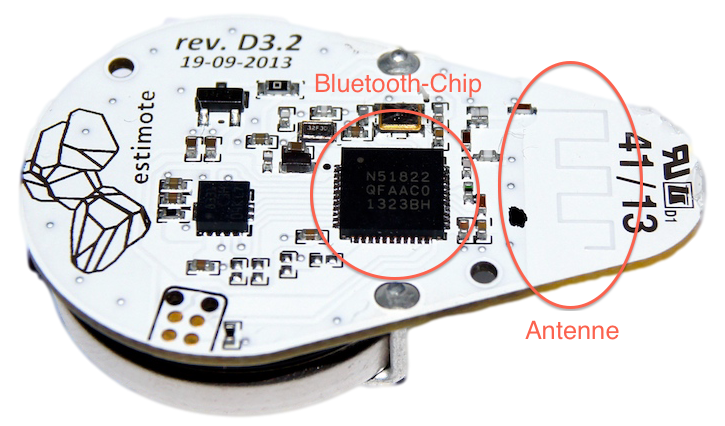
\includegraphics[scale=0.25]{estimote-beacon-inside-annotation}
	\caption{Aufbau des estimote-Beacons}
	\label{estimote-beacon-inside-annotations}
\end{figure}



%%%%%%%%%%%%%%%%%%%%%%%%%%%%%%%%%%%%%%%%%%%%%%%%%%%%%%%%%%%%
\section{iOS, OS X und Xcode}
\label{sec:technologies:iosandxcode}
%%%%%%%%%%%%%%%%%%%%%%%%%%%%%%%%%%%%%%%%%%%%%%%%%%%%%%%%%%%%
Für die Entwicklung der Applikation zur Indoor Positionierung war eine der Vorgaben, dass diese für iOS programmiert werden soll.
Daher waren drei Dinge zwingend notwendig: ein Mac, Xcode und ein iOS-Gerät.

Für die Entwicklung setzte ich deshalb auf ein Macbook Pro mit installiertem Xcode und als iOS-Gerät setzte ich ein iPhone 5 ein.
Als minimale iOS-Version musste iOS 7 verwendet werden, da die iBeacon-Features des CoreLocation-Frameworks (mehr dazu im Kapitel \ref{sec:technologies:corelocation}) erst ab dieser Version zur Verfügung stehen.


%%%%%%%%%%%%%%%%%%%%%%%%%%%%%%%%%%%%%%%%%%%%%%%%%%%%%%%%%%%%
\section{CoreLocation-Framework}
\label{sec:technologies:corelocation}
%%%%%%%%%%%%%%%%%%%%%%%%%%%%%%%%%%%%%%%%%%%%%%%%%%%%%%%%%%%%
Das Core Location-Framework erlaubt es aktuelle Positions- und Richtungsinformationen eines Gerätes zu bestimmen.
Die Positionsbestimmung lässt sich dabei über verschiedene Werte und Sensoren bestimmen und auch der Grad der Genauigkeit ist variabel.
Auch die Aktualiserungsrate der Position lässt sich festlegen, wobei eine höhere Aktualisierungsrate auch gleichbedeutend mit einem höherem Akkuverbrauch ist.

Bei der Genauerigkeit gibt es dabei verschiedene Konstanten, die die gewollte Genauigkeit bestimmen. 


    \begin{table}[htb!]
      \centering
      \begin{tabular}{l p{6cm}}
        Konstante & Erwartete Genauigkeit \\ \\
		\emph{kCLLocationAccuracyThreeKilometers} & Genauigkeit auf 3 Kilometer \\
		\emph{kCLLocationAccuracyKilometer} & Genauigkeit auf 1 Kilometer \\
		\emph{kCLLocationAccuracyHundredMeters} & Genauigkeit auf 100 Meter \\
		\emph{kCLLocationAccuracyNearestTenMeters} & Genauigkeit auf 10 Meter \\
		\emph{kCLLocationAccuracyBest} & Höchstmögliche Genauigkeit \\
		\emph{kCLLocationAccuracyBestForNavigation} & Höchstmögliche Genauigkeit und weitere Sensordaten für die Navigation
      \end{tabular}
      \caption{Mögliche Optionen der Positionsgenauigkeit}
      \label{tbl:positionaccuracy}
    \end{table}
	
Diese Genauigkeiten beziehen sich hauptsächlich auf die Positionierung mittels GPS und sind daher für die Indoor Positionierung nur bedingt geeignet.


Eine weitere Funktion des Core Location-Frameworks ist die Bestimmung der Himmelsrichtungen. Durch den eingebauten Kompass in den neueren iOS-Geräten ist es möglich, die aktuelle Ausrichtung des Gerätes zu bestimmen. Dies ist im Bezug auf die Indoor Navigation hilfreich, da diese Informationen in die Positionsbestimmung einbezogen werden können.
Des Weiteren erlaubt diese Funktion eine dynamische Ausrichtung der Karte, abhängig davon in welche Richtung man momentan schaut.


Die für uns zentrale Funktion dieses Frameworks ist die Erkennung von iBeacons und die Funktionen zur Verarbeitung der gesendeten Daten.
Damit können Beacons anhand ihres UUID erkannt werden und einer Region zugeordnet werden. Die genaue Funktionsweise wird in Kapitel \ref{sec:technologies:corelocation:ibeaconsapi}.

Die Funktionen zum Positionsupdate und zur Erkennung der Beacons werden dabei im \emph{LocationManager} verwaltet.
In der \emph{LocationManagerDelegate} lassen sich dabei die Aktionen bestimmen, welche bei verschiedenen Events ausgeführt werden.

In Listing \ref{lst:locationmanager_objc} wird die Initialisierung eines LocationManager gezeigt, welcher eine Genauigkeit von einem Kilometer haben soll und bei Positionsänderungen von mehr als 500 Metern aktualisiert wird.

  \begin{listing}[htb!]
    \insertminted{objc}{code_examples/locationManager.m}
    \caption{Beispielinitialisierung für einen LocationManager.}
    \label{lst:locationmanager_objc}
  \end{listing}

%%%%%%%%%%%%%%%%%%%%%%%%%%%%%%%%%%%%%%%%%%%%%%%%%%%%%%%%%%%%
\subsection{iBeacons-API}
\label{sec:technologies:corelocation:ibeaconsapi}
%%%%%%%%%%%%%%%%%%%%%%%%%%%%%%%%%%%%%%%%%%%%%%%%%%%%%%%%%%%%
Seit der iOS Version 7 wurde das Core Location Framework um die Beacon-Funktionen erweitert. 
Dazu wurden zwei neue Klassen geschaffen. Einmal die \emph{CLBeacon}-Klasse, welche ein iBeacon repräsentiert und alle zur verfügungsteheneden Informationen enthält und zum anderen die \emph{CLBeaconRegion}-Klasse, welche eine Region mit mehreren Beacons, abhängig von ihrem UUID, beschreibt.

Die \emph{CLBeacon}-Klasse besteht dabei lediglich aus Propertys mit den gegenbenden Beacon-Informatinen, wie \emph{UUID}, \emph{major}, \emph{minor}, \emph{accuracy}, \emph{proximity} und \emph{rssi}.

Die \emph{CLBeaconRegion}-Klasse ist etwas umfangreicher und bestimmt letztendlich, nach welchen Beacons gesucht werden soll.
Dabei ist es möglich die Region in verschiedene Genaugikeitsstufen einzuteilen.


\emph{initWithProximityUUID:identifier:}\begin{quote}
	Die Region ist nur abhängig von dem UUID und dem Identifier der Beacons, das heißt es werden alle Beacons mit dem gegebenen UUID gesucht.
\end{quote}
\emph{initWithProximityUUID:major:identifier:}\begin{quote}
	Die Region ist abhängig von dem UUID, dem Identifier und dem Major-Wert der Beacons. Es werden nur Beacons eines bestimmten Major-Wertes gesucht.
\end{quote}
\emph{initWithProximityUUID:major:minor:identifier:}\begin{quote}
	Die Region ist abhängig von dem UUID, dem Identifier, dem Major-Wert und dem Minor-Wert der Beacons. Es werden nur Beacons mit passendem Major und Minor-Wert gesucht. In diesem Fall ist bei mehreren erkannten Beacons keine Unterscheidung mehr möglich.
\end{quote}


Mittels des Location Manager lässt sich dann gezielt nach bestimmten Regionen suchen.


%%%%%%%%%%%%%%%%%%%%%%%%%%%%%%%%%%%%%%%%%%%%%%%%%%%%%%%%%%%%
\section{MapBox}
\label{sec:sec:technologies:mapbox}
%%%%%%%%%%%%%%%%%%%%%%%%%%%%%%%%%%%%%%%%%%%%%%%%%%%%%%%%%%%%
MapBox ist ein Online-Karten Anbieter, welcher es erlaubt eigene Karten zu erstellen und über ihren Service bereitzustellen. 
Die Karten werden dabei vom OpenStreetMap Projekt bereitgestellt und MapBox erlaubt es diese Karten grafisch zu überarbeiten, um zum Beispiel das Farbschema zu ändern, eigene Markierungen zu setzen oder auch eigene Layer über die Karte zu legen.
Ausserdem stellt MapBox ein SDK für iOS bereit, welche es erlaubt diese individuell angepassten Karten in iOS anzuzeigen und gleichzeitig die Funktionen des native MapKit-Framework mit sich bringt. Ausserdem besitzt MapBox eine größere Flexibilität im Bezug auf die individuelle Anpassung und den Offline-Betrieb, das die Karten direkt auf dem Gerät gespeichert werden können.

Bisher ist die Unterstützung von Indoor-Karten jedoch noch nicht gegeben, sodass man hierbei nicht auf schon vorhandenes Kartenmaterial zurückgreifen kann.

Google hat mit Google Maps Indoor bereits einen Dienst gestartet, welcher Gebäudepläne in Google Maps integriert, bisher handelt es sind jedoch dabei hauptsächlich um öffentliche Gebäude in US-amerikanischen Städten. Das hinzufügen von neuen Gebäudeplänen ist nur bei öffentlichen Gebäuden möglich und nicht für den privaten Gebrauch vorgesehen, daher konnte ich nicht darauf zurückgreifen.

Die Indoor-Karten mussten daher selbst erstellt und in ein, von Mapbox verständliches Format umgewandelt werden.
Die Ausgangsdatei ist dabei eine Bilddatei mit der Karte des Innenraumes, welche selbst angefertigt wurde. Dieses Bild der Karte muss nun in ein passendes Geo-Format überführt werden. 
Dazu wurde ein von ''Tom MacWright'' (\citet{jpgtogeo}) bereitgestellte Python-Script verwendet, welches JPEG Dateien in GeoTIFF Dateien umwandelt. Die GeoTiff Datei speichert neben den eigentlichen Bilddaten noch Koordinaten für die Georeferenzierung. \citet{geotiff}

Mit diesem GeoTIFF ist es nun möglich eine eigene Karte zu erstellen, welche letztendlich auf dem iOS-Gerät ausgegeben wird.
Dafür stellt MapBox das Programm \emph{TileMill} zur Verfügung. Dieses erlaubt es eigene Karten zu erstellen und zu bearbeitet. Die erstellte Karte kann anschließend in verschiedenen Formaten exportiert werden. 
TileMill bietet einen Import von GeoTIFF-Dateien an, sodass unsere Karte direkt eingefügt werden kann.

\begin{figure}[htb!]
	\centering
	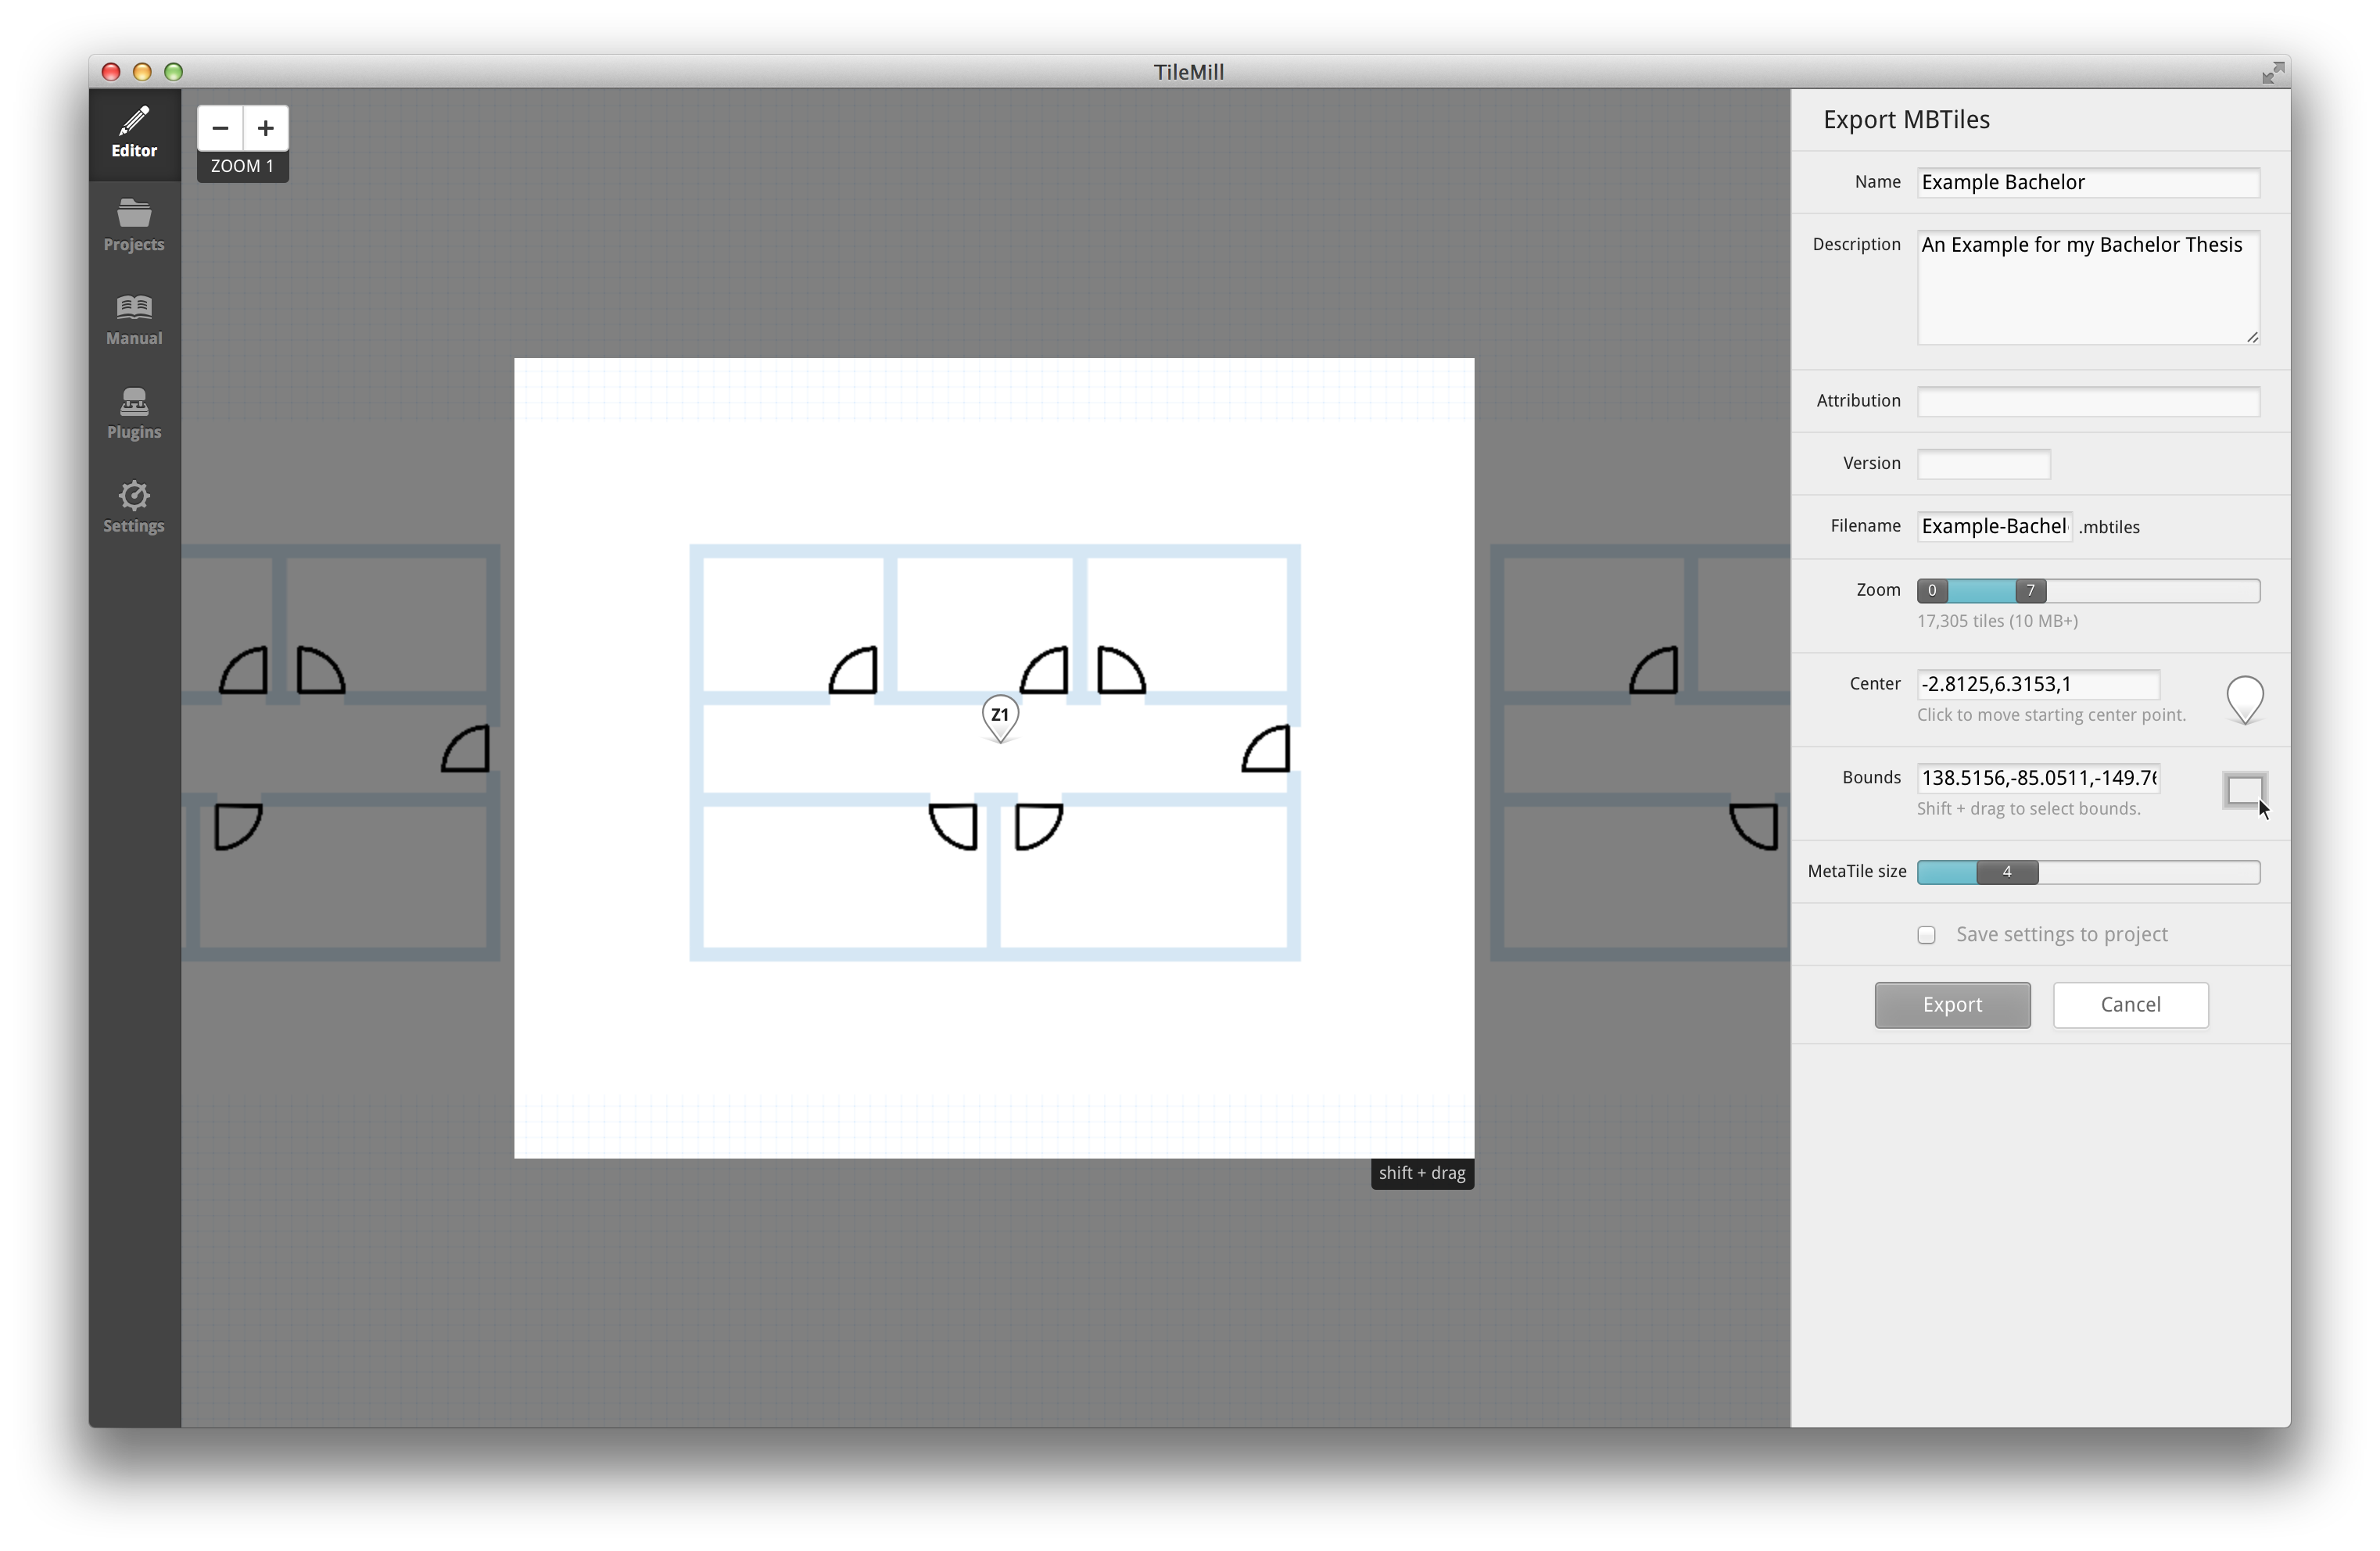
\includegraphics[scale=0.25]{tilemill-example}
	\caption{Karte in TileMill}
	\label{tilemill-example}
\end{figure}

TileMill erlaubt es nun die eingefügte Karte weiter zu bearbeiten, was in unserem Fall jedoch nicht nötig ist.
Der nächste Schritt ist es die Karte in ein für iOS beziehungsweise das Mapbox SDK, verstädnliches Format zu überführen.
Dazu wird die Karte als \emph{mbtiles} exportiert. Dies ist ein von Mapbox entwickeltes Dateiformat, welches die Karte in Kacheln speichert um das Laden der einzelnen Kartenabschnitte bei größeren Karten zu beschleunigen, sodass nicht die komplette Karte geladen werden muss, sondern nur die benötigten Kacheln.

Die erzeugte \emph{.mbtiles}-Datei lässt sich nun in die iOS Appikation einbinden und über das SDK auf dem iOS-Gerät ausgeben. In Abbildung \ref{mapbox-map-ios} sieht man die Ausgabe einer Karte auf dem iPhone 5.

\begin{figure}[htb!]
		\centering
	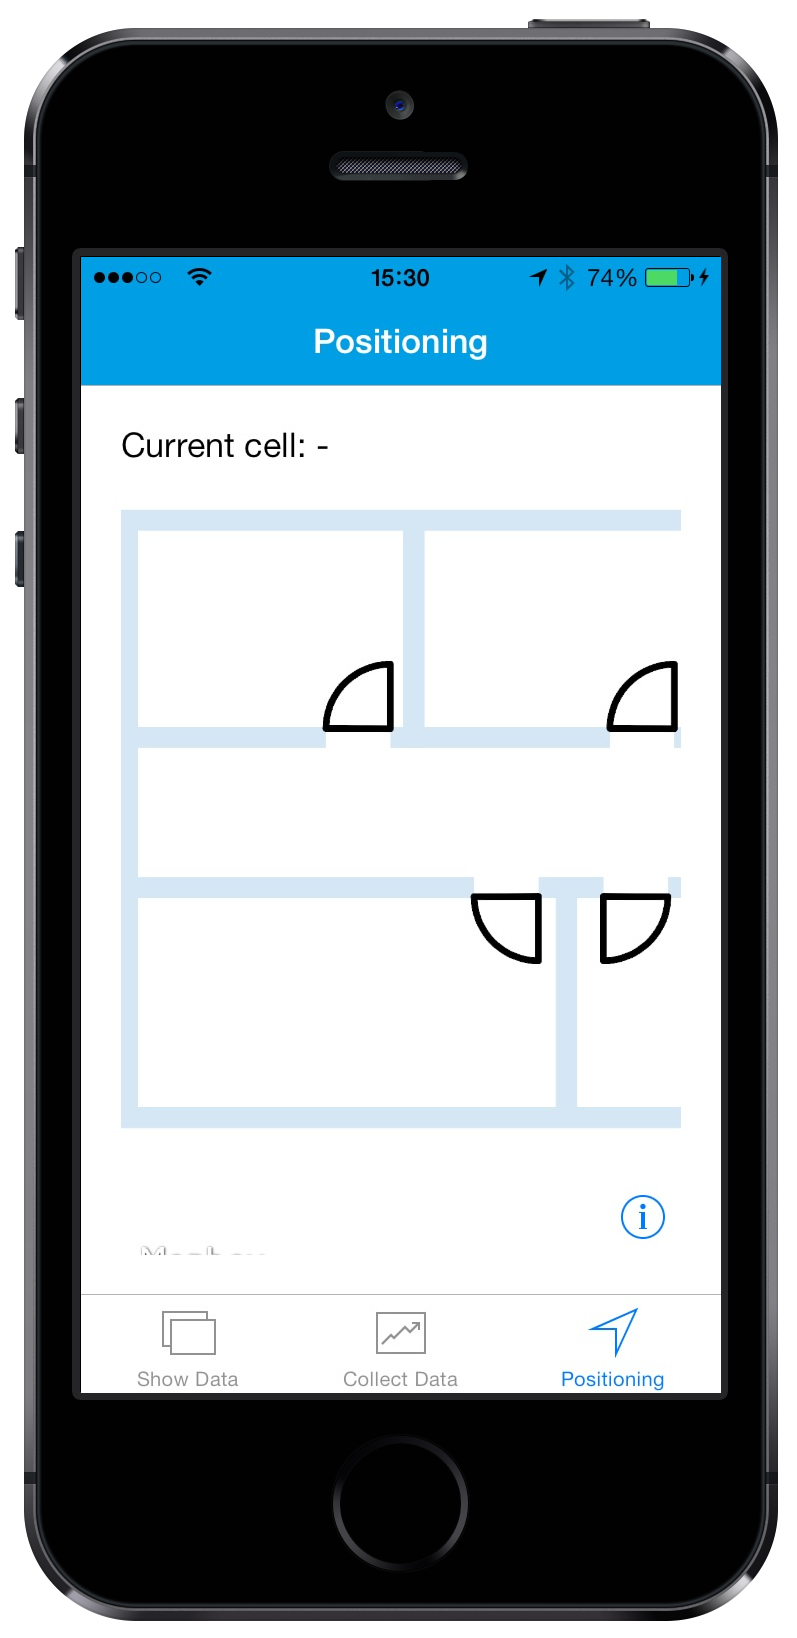
\includegraphics[scale=0.25]{mapbox-map-ios-mockup}
	\caption{Kartenausgabe mittels Mapbox SDK auf dem iPhone}
	\label{mapbox-map-ios}
\end{figure}

Diese Karte wird offline auf dem Gerät gespeichert, es ist also keine Internetverbindung nötig und diese anzuzeigen.

Für die Anzeige auf dem Gerät ist es zunächst nötig einen \emph{RMMapView} anzulegen, welcher für die Ausgabe der Karte verantwortlich ist und gleichzeitig die gewohnten MapView-Features wie zum Beispiel \emph{Pinch-to-Zoom} oder die automatische Ausrichtung auf den Mittelpunkt mit sich bringt.
Da wir unser eigenes Kartenmaterial verwendet ist es zudem nötig die Quelle für Kartendaten des MapViews zu ändern, da ansonsten die Daten des OpenStreetMap-Projekts genutzt werden. Dazu wird eine eigene \emph{RMTileSource} angelegt, welche die zuvor generierten \emph{mbtiles} läd und dem MapView zur Verfügung stellt. 
In Listing \ref{lst:RMMapView_objc} wird diese Inintialisierung gezeigt.

\begin{listing}[htb! breaklines=true]
    \insertminted{objc}{code_examples/RMMapView.m}
    \caption{Initialisierung des MapView mit eigenem Kartenmaterial}
	\label{lst:RMMapView_objc}
\end{listing}

%%%%%%%%%%%%%%%%%%%%%%%%%%%%%%%%%%%%%%%%%%%%%%%%%%%%%%%%%%%%
\subsection{Weitere API's}
\label{sec:technologies:iosandxcode:otherapis}
%%%%%%%%%%%%%%%%%%%%%%%%%%%%%%%%%%%%%%%%%%%%%%%%%%%%%%%%%%%%


%%%%%%%%%%%%%%%%%%%%%%%%%%%%%%%%%%%%%%%%%%%%%%%%%%%%%%%%%%%%
\section{CoreData-Framework}
\label{sec:technologies:coredata}
%%%%%%%%%%%%%%%%%%%%%%%%%%%%%%%%%%%%%%%%%%%%%%%%%%%%%%%%%%%%
Core Data ist ein Framework für die Organisation und Speicherung von Daten in einem Entity-Realationship-Modell.
Core Data vereinfacht die Speicherung und den Zugriff auf die Daten, da es für jede Entity ein eigenes Objekt erstellt.
Die eigentliche Datenspeicherung sieht dabei drei Verschiedene speichermöglichkeiten vor, entweder als Binärdatei, als XML-Datei oder in einer SQLite-Datenbank. 
Nachdem eine Core Data-Datenbank erstellt wurde, benötigt man zunächst ein \emph{NSManagedObjectContext}, welcher Lese- und Schreibzugriffe auf die Datenbank steuert und verwaltet.
Objekte aus der Datenbank werden durch \emph{NSManagedObject} repräsentiert. Nach dem anlegen der Datenbank ist es jedoch auch möglich sich direkt eigene Klasse für die einzelnen Datenbank-Objekte erzeugen zu lassen, welche alle Attribute und Funktionen der einzelnen Objekte und Verbindungen beinhalten und somit den Zugriff enorm erleichtern.

Um auf die Daten zuzugreifen und diese zu verändern ist es zunächst nötig sie aus der Datenbank zu extrahieren. Dazu verwendet man einen \emph{NSFetchRequest}, welcher Objekte nach bestimmten Kriterien aus der Datenbank holt.
Dabei ist es möglich den \emph{NSFetchRequest} zu spezialisieren und so nur Objekte mit bestimmten Eigenschaften anzuzeigen.
Dafür verwendet man ein \emph{NSPredicate}, welches umfangreiche Vergleiche von Attributen und logische Operationen erlaubt.

\begin{listing}[htb! breaklines=true]
    \insertminted{objc}{code_examples/NSFetchRequest.m}
    \caption{Fetch Request für alle Objekte die mit Nachnamen ''muller'' heißen und mehr als 3000 Euro im Monat verdienen}
	\label{lst:NSFetchRequest_objc}
\end{listing}

Als Rückgabewert erhält man ein Array mit allen Objekten auf die die gegebenen Kriterien zutreffen.
